\subsection{Person 3 – SUS 85,0}
\textbf{Zur Person:}\\
Medizin-Student, 24 Jahre alt

\textbf{Beobachtung:}
\begin{enumerate}
\item Zeichnen Sie frei für etwa 2 Minuten.
\begin{itemize}
\item Präzision meist sehr gut; kleinere Probleme beim Setup mit Doppel-Erkennung.
\item Leichter Delay, aber nicht gravierend.
\item Schrift problemlos.
\end{itemize}

\item Löschen Sie Ihre Zeichnung vollständig.
\begin{itemize}
    \item Alles löschen problemlos; selbsterklärend.
\end{itemize}

\item Laden Sie die PDF-Datei mit dem Grundriss \texttt{Hospital\_Floor\_Plan.pdf} hoch.
\begin{itemize}
    \item Alles problemlos.
\end{itemize}

\item Ändern Sie die Stiftfarbe auf Rot.
\begin{itemize}
    \item Funktion bereits beim freien Zeichnen allerdings nicht absichtlich; Änderung eventuell Drop-down-Indikator wünschenswert.
\end{itemize}

\item Suchen Sie \texttt{BEDROOM3} und zeichnen Sie einen Tisch links vom Bett.
\begin{itemize}
    \item Funktion ausgeführt; kleinere Probleme wegen Bugs in den PDF-Controls.
\end{itemize}

\item Radieren Sie den Tisch und zeichnen Sie ihn rechts vom Bett.
\begin{itemize}
    \item Gewohnt von iPad: PDF-Linie, Radiergummi und Smart-Eraser Funktion.
    \item Sonst alles ok.
\end{itemize}

\item Zeichnen Sie die Abmessungen 1\,m $\times$ 1\,m und schreiben Sie «table» hinein.
\begin{itemize}
    \item Keine Probleme.
\end{itemize}

\item Speichern Sie den Plan auf Ihrem Laptop.
\begin{itemize}
    \item Keine Probleme.
\end{itemize}
\end{enumerate}

\clearpage

\textbf{SUS-Antworten (Bild):}
\begin{center}
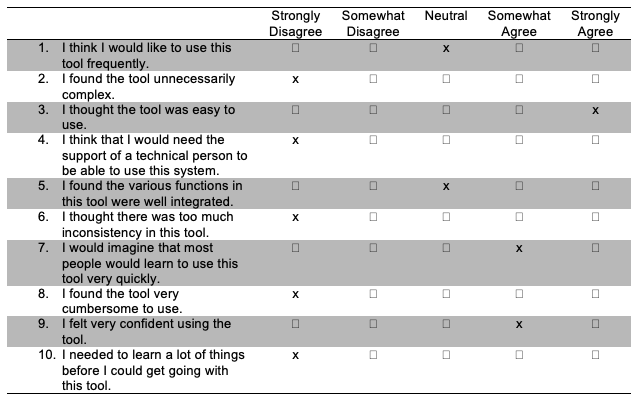
\includegraphics[width=0.95\textwidth]{graphics/sus_person3.png}
\end{center}

\textbf{Follow-up:}  
\begin{enumerate}
    \item \textbf{Was hat Ihnen am Tool am besten gefallen?}
    \begin{itemize}
        \item Freiheit, auf beliebiger Fläche zu zeichnen und damit verbundene Flexibilität.
    \end{itemize}

    \item \textbf{Gab es etwas, das verwirrend oder schwierig zu bedienen war?}
    \begin{itemize}
        \item Tracking-Fehler (Zacken-Bug).
        \item PDF-Controls teilweise verwirrend.
        \item Reset-Button löscht PDF-Elemente mit.
    \end{itemize}

    \item \textbf{Fehlt etwas, das Sie erwartet oder gerne gehabt hätten?}
    \begin{itemize}
        \item Rückgängig-Funktion (Undo).
        \item Wiederherstellen-Funktion.
        \item Lasso-Löschen, Duplizieren und Verschieben von Elementen.
        \item Touch-Input-Unterstützung.
    \end{itemize}

    \item \textbf{Haben Sie Vorschläge, wie das Tool verbessert werden könnte?}
    \begin{itemize}
        \item Bessere Projektion der Unterlagen.
        \item Details besser lesbar machen (bedingt durch Setup).
        \item Fehlende Funktionen, die erwartet werden, implementieren (z.B. Undo, Lasso, Duplizieren).
    \end{itemize}
\end{enumerate}

\clearpage